Electrons and positrons pose a special case due to their low mass ($m_{e^{\pm}} \approx
511$~keV/c$^2$, $m_{\mu} \approx 106$~MeV/c$^2$). In addition to loss of energy through ionisation
and excitation, the loss of energy through bremsstrahlung gain in importance:

\[-\left(\frac{dE}{dx}\right)_{\text{tot}} = -\left(\frac{dE}{dx}\right)_{\text{coll}}
-\left(\frac{dE}{dx}\right)_{\text{rad}} \]

The Bethe-Bloch formula has to be modified in the case of energy loss through ionisation and
excitation. The loss of energy through ionisation increase logarithmically with $E$ and linearly
with $Z$, whereas the energy loss through bremsstrahlung increases linearly with $E$ and to the
square of $Z$. For high energies (> 1~GeV), bremsstrahlung is the dominating process. 

\begin{figure}[H]
	\centering
	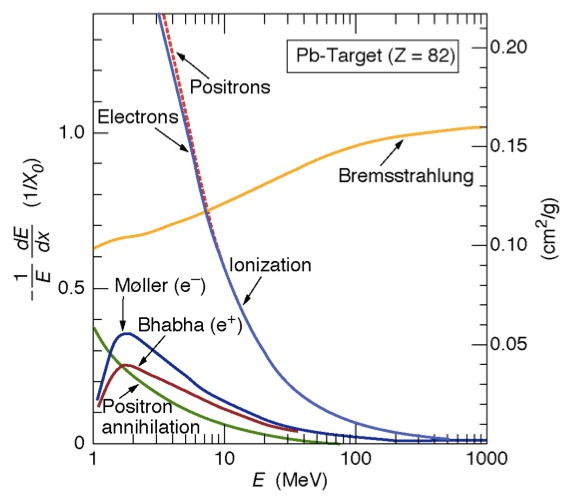
\includegraphics[width=0.5\textwidth]{energieverlust.jpg}
	\caption{}
	\label{}
\end{figure}
